\documentclass[12pt,letterpaper]{article}

\usepackage{graphicx}
\author{Pantita Palittapongarnpim}
\title{Documentation for Modular Version of Quantum Optimization Program}
\begin{document}

\maketitle

The aim of this version of the program is to streamline the implementation of different optimization algorithms to a problem. 
From the user end, the switching between algorithms is aimed to be as easy as specifying one line of code in the main function.

\section{Overall Structure}

\begin{figure}[h]
\centering
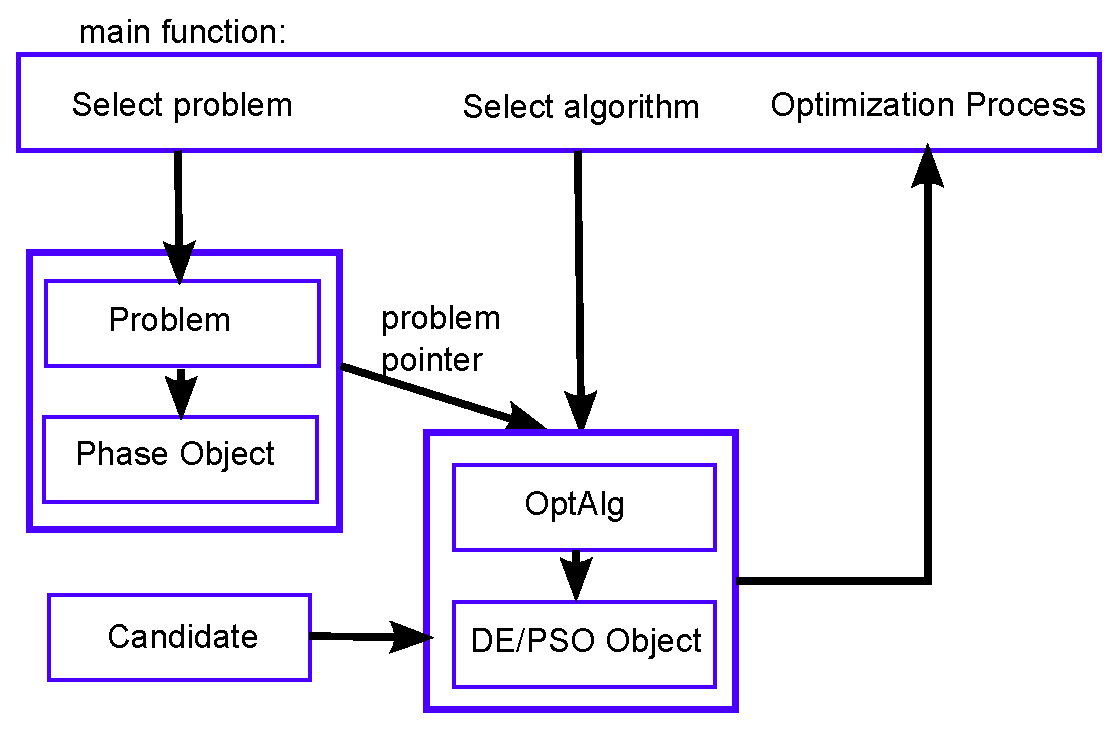
\includegraphics[width=0.7\linewidth]{diagram}
\caption{Diagram of how classes are used in the program.}
\label{fig:diagram}
\end{figure}

The structure is inspired by the one used in PaGMO library which accesses the problem and the optimization algorithm through base classes.
The main difference is between our program and PaGMO lies in the parallelization of the optimization algorithm.  
PaGMO initializes multiple optimization algorithms, one per processor, and exchanges the candidates between algorithms to aid the searching of the near optimal solution.
Our program initializes one optimization algorithm that uses multiple processors to compute the solution candidates. 
The reason the program is structured in this way is because our fitness function is computationally expensive, and therefore the processor power has to be directed towards computing the fitness function in order to gain speed up.
 
The program contains three components.
The main function is where the optimization algorithm is put together. 
The \textit{OptAlg} class is the base class for modules of optimization algorithms and memory management functions. 
DE and PSO inherited \textit{OptAlg} class and their specific update rules are accessed through virtual functions in \textit{OptAlg} class. 
These classes are also where the code is parallelized using MPI. 
The third part of the program is the \textit{Problem} class which is the base class that contains virtual functions for the fitness functions of a specific problem. 
The \textit{Problem} class is not parallelized.

\section{Classes}

This part of the documentation contains brief descriptions of the three main classes: \textit{Candidates}, \textit{OptAlg}, and \textit{Problem}.
Since these classes contain many functions and most of them have names that are self-explanatory, I will limit this section to discussing the functions and variables whose role might not be obvious at first glance.

\subsection{Candidate Class}

Candidate class contains the variables and functions to initialize, update, and read values stored by a solution candidate.
This class is used by \textit{OptAlg} class to store the solutions and the fitness values.
 
\noindent Position variables:

\begin{description}
\item[\textit{can\underline{ }best}] stores the candidate solution for DE and personal best position for PSO.
\item[\textit{contender}] stores the offspring for DE and current position for PSO.
\item[\textit{global\underline{ }best}] stores the global best position for PSO and used by \textit{OptAlg} class to find the solution to be output to user.
\end{description}
       
\noindent Velocity variable:

\begin{description}
\item[\textit{velocity}] is only initialized for PSO to store current velocity.
\end{description} 

\subsection{Base Classes}

\subsubsection{Problem Class (problem.h): base class for optimization problems}
 
        Virtual functions:
 		
 		\begin{description}
 		\item[\textit{fitness}]
 		\item[\textit{avg\underline{ }fitness}]
 		\end{description}
 
            \textit{avg\underline{ }fitness} is meant to compute the fitness value from \textit{K} number of samples set by the user. \textit{fitness} can be written to compute from only one sample or from an ensemble with a pre-calculated size not in direct control of the user. 
            Having two fitness functions available also allows us to test the solution learned under one condition in another such as the case of testing feedback policies for lossless system in lossy system.
       
       \noindent Class function:
       \begin{description}
       \item[\textit{modulo}] function bounds the solution.
       \item[\textit{normalize}] function normalizes the solution.
       \end{description}
       
        \noindent Variables:
        
        \textit{Problem} class also contains the arrays storing the lower bound and the upper bound of each variable. 
        These arrays are initialized by classes written for specific problems which inherits the \textit{Problem} class.   

\subsubsection{OptAlg Class (mpi\underline{ }optalg.h): base class for modules of optimization algorithms.}

This class takes the problem pointer as input for instantiation and contains most of the modules needed for any global optimization algorithm such as candidate initialization functions, functions for final selection of solution, functions for setting and checking success criteria for the optimization, and other memory management functions.
 
       \noindent Class functions:
        
        \begin{description}
        \item[\textit{Final\underline{ }select}] selects the candidate with the highest fitness value by comparing the fitness stored by each candidate.
        \item[\textit{avg\underline{ }Final\underline{ }select}] selects the candidate with the highest mean fitness value calculated from \textit{repeat} number of computation. This function is useful for noisy fitness function in which the fitness value is better represented by the mean.
        \end{description}
 
        \noindent Virtual functions: these are functions that are specific to the optimization algorithm.
        
        \begin{description}
        \item[\textit{combination}] function contains the rules of creating new solution candidate for the next iteration.
        \item[\textit{selection}] function contains the rules for deciding whether the new candidate should replace the old one. This function is currently written for maximization.
        \item[\textit{put\underline{ }to\underline{ }best}] function performs the first calculation of the candidates and update the results to respective memories. For PSO, this function also finds the global best position.
        \item[\textit{fit\underline{ }to\underline{ }global}] function is for DE algorithm to put its current solutions to the memories for global solutions because the \textit{Final\underline{ }select}  and \textit{avg\underline{ }Final\underline{ }select} select from the global solutions.
        \end{description}
        
        The parameters of the optimization algorithms are initialized with fixed values, but they can be changed using \textit{write\underline{ }param} function.

\section{Known Issues with Current Version}

\begin{enumerate}
\item Switching between standard and complex data types

The program is also designed to streamline the process of inputting different problems. 
However, because the operators for complex type variables do not always match ones for the standard data types such as \textit{double} or \textit{int}, the code for certain functions needed to be modified to accommodate complex data types. 
These functions are:
 \begin{itemize}
 \item \textit{Problem} class: \textit{modulo} function, \textit{normalize} function.
 \item \textit{OptAlg} class: \textit{Init\underline{ }previous} function.  
 \end{itemize}
 
\item Input state generation in phase measurement problem

The input state for the phase measurement problem can only be generated reliably to 100 photons, although the new algorithm has eliminated the \textit{\#inf} components in states with of than 98 photons. 
Pushing beyond 100 photons results in unnormalized states. This problem might be eliminated by using GMP library, which can create data types of arbitrary precision, but this potential solution has yet to be tested. 

\item Computational overhead

The program is tested from 4 to 65 photons and at 100 photons. The current roadblock is the computational overhead which results in the time-cost of 642 seconds per iteration at 100 photons. Further optimization is underway to resolve this issue.

\end{enumerate}


\end{document}